\documentclass[tikz,border=6pt]{standalone}
\usetikzlibrary{arrows.meta,positioning,calc,circuits.logic.US}
\makeatletter
\AtBeginDocument{\global\let\pgf@selectfontorig\relax}
\makeatother

\tikzset{
  nodebox/.style={draw=black, rounded corners=4pt, very thick, fill=gray!4,
    minimum width=10mm, minimum height=7mm, align=center, inner sep=2pt},
  circuitbox/.style={draw=black, rounded corners=4pt, very thick, fill=gray!4,
    minimum width=53mm, minimum height=35mm, align=center, inner sep=5pt},
  regbox/.style={draw=black, very thick, rounded corners=2pt, fill=white,
    minimum width=9mm, minimum height=7mm, align=center, inner sep=1pt},
  initial/.style={-Latex, very thick},
  edge/.style={-Latex, thick, shorten >=3pt, shorten <=3pt},
  wire/.style={-Latex, thick},
  plainwire/.style={thick},
  gate/.style={draw, very thick, logic gate inputs=nn, minimum width=11mm, minimum height=8mm},
  onegate/.style={draw, very thick, minimum width=9mm, minimum height=7mm},
  gatetext/.style={font=\fontsize{5}{6}\selectfont, inner sep=0pt},
  dot/.style={circle, fill=black, inner sep=1.2pt}
}

\newcommand{\initarrow}[2]{\draw[initial] #1 -- (#2);}

\newcommand{\commonpins}[1]{
  \node at (2.2,2.8) {\bfseries\large $#1$};
  \node[circuitbox] at (2.2,.55) {};
  \node[anchor=east] (#1x) at (-.55,1.55) {$x$};
  \node[regbox] (#1reg) at (4.10,-.2) {$r$};
  \node[anchor=west] (#1y) at (5.05,1.55) {$y$};
  \coordinate (#1rp) at (#1reg.west);
  \draw[plainwire] (#1reg.east) -- (4.65,-.2) -- (4.65,-1) -- (.95,-1) -- (.95,.05);
}

\begin{document}
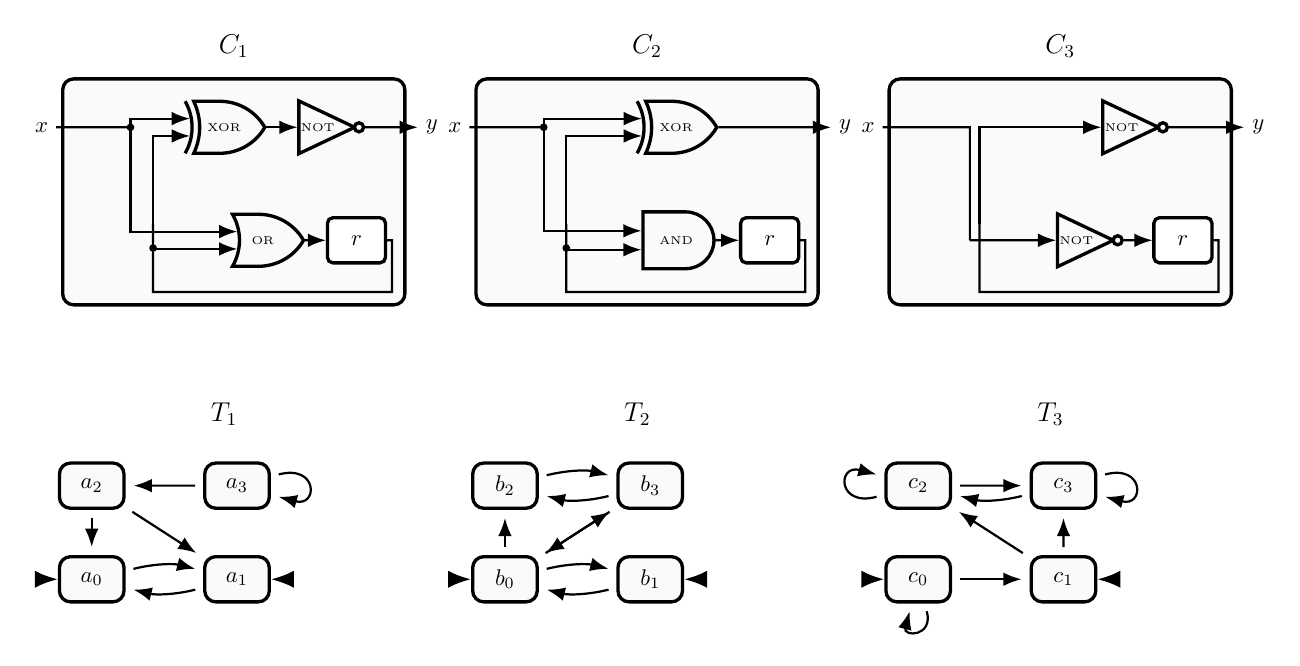
\begin{tikzpicture}[scale=.82, transform shape]
  \begin{scope}[shift={(0,5.45)}]
    \commonpins{C_1}
    \node[dot] at (.95,-.32) {};
    \node[xor gate US, gate] (c1xor) at (2.05,1.55) {};
    \node[not gate US, onegate] (c1not) at (3.5,1.55) {};
    \node[or gate US, gate] (c1or) at (2.65,-.2) {};
    \node[gatetext] at (c1xor.center) {XOR};
    \node[gatetext] at (c1not.center) {NOT};
    \node[gatetext] at (c1or.center) {OR};
    \draw[plainwire] (C_1x) -- (.6,1.55);
    \node[dot] at (.6,1.55) {};
    \draw[wire] (.6,1.5) |- (c1xor.input 1);
    \draw[wire] (.95,.05) |- (c1xor.input 2);
    \draw[wire] (c1xor.output) -- (c1not.input);
    \draw[wire] (c1not.output) -- (C_1y);
    \draw[wire] (.6,1.55) |- (c1or.input 1);
    \draw[wire] (.95,.05) |- (c1or.input 2);
    \draw[wire] (c1or.output) -- (C_1rp);
  \end{scope}

  \begin{scope}[shift={(6.4,5.45)}]
    \commonpins{C_2}
    \node[dot] at (.95,-.32) {};
    \node[xor gate US, gate] (c2xor) at (2.65,1.55) {};
    \node[and gate US, gate] (c2and) at (2.65,-.2) {};
    \node[gatetext] at (c2xor.center) {XOR};
    \node[gatetext] at (c2and.center) {AND};
    \draw[plainwire] (C_2x) -- (.6,1.55);
    \node[dot] at (.6,1.55) {};
    \draw[wire] (.6,1.5) |- (c2xor.input 1);
    \draw[wire] (.95,.05) |- (c2xor.input 2);
    \draw[wire] (c2xor.output) -- (C_2y);
    \draw[wire] (.6,1.55) |- (c2and.input 1);
    \draw[wire] (.95,.05) |- (c2and.input 2);
    \draw[wire] (c2and.output) -- (C_2rp);
  \end{scope}

  \begin{scope}[shift={(12.8,5.45)}]
    \commonpins{C_3}
    \node[not gate US, onegate] (c3ynot) at (3.15,1.55) {};
    \node[not gate US, onegate] (c3rnot) at (2.45,-.2) {};
    \node[gatetext] at (c3ynot.center) {NOT};
    \node[gatetext] at (c3rnot.center) {NOT};
    \draw[plainwire] (C_3x) -- (.8,1.55) -- (.8,-.2);
    \draw[wire] (.8,-.2) -- (c3rnot.input);
    \draw[wire] (c3rnot.output) -- (C_3rp);
    \draw[wire] (.95,.05) |- (c3ynot.input);
    \draw[wire] (c3ynot.output) -- (C_3y);
  \end{scope}

  \begin{scope}[shift={(0,0)}]
    \node at (2.05,2.55) {\bfseries\large $T_1$};
    \node[nodebox] (a0) at (0,0) {$a_0$};
    \node[nodebox] (a1) at (2.25,0) {$a_1$};
    \node[nodebox] (a2) at (0,1.45) {$a_2$};
    \node[nodebox] (a3) at (2.25,1.45) {$a_3$};
    \initarrow{(-.75,0)}{a0.west}
    \initarrow{(3,0)}{a1.east}
    \draw[edge,bend left=14] (a0) to (a1);
    \draw[edge,bend left=14] (a1) to (a0);
    \draw[edge] (a2) -- (a0);
    \draw[edge] (a2) -- (a1);
    \draw[edge] (a3) -- (a2);
    \draw[edge,loop right,looseness=7] (a3) to (a3);
  \end{scope}

  \begin{scope}[shift={(6.4,0)}]
    \node at (2.05,2.55) {\bfseries\large $T_2$};
    \node[nodebox] (b0) at (0,0) {$b_0$};
    \node[nodebox] (b1) at (2.25,0) {$b_1$};
    \node[nodebox] (b2) at (0,1.45) {$b_2$};
    \node[nodebox] (b3) at (2.25,1.45) {$b_3$};
    \initarrow{(-.75,0)}{b0.west}
    \initarrow{(3,0)}{b1.east}
    \draw[edge] (b0) -- (b2);
    \draw[edge] (b0) -- (b3);
    \draw[edge,bend left=14] (b1) to (b0);
    \draw[edge,bend left=14] (b0) to (b1);
    \draw[edge,bend left=14] (b2) to (b3);
    \draw[edge,bend left=14] (b3) to (b2);
    \draw[edge] (b3) -- (b0);
  \end{scope}

  \begin{scope}[shift={(12.8,0)}]
    \node at (2.05,2.55) {\bfseries\large $T_3$};
    \node[nodebox] (c0) at (0,0) {$c_0$};
    \node[nodebox] (c1) at (2.25,0) {$c_1$};
    \node[nodebox] (c2) at (0,1.45) {$c_2$};
    \node[nodebox] (c3) at (2.25,1.45) {$c_3$};
    \initarrow{(-.75,0)}{c0.west}
    \initarrow{(3,0)}{c1.east}
    \draw[edge,loop below,looseness=7] (c0) to (c0);
    \draw[edge] (c0) -- (c1);
    \draw[edge] (c1) -- (c2);
    \draw[edge] (c1) -- (c3);
    \draw[edge,loop left,looseness=7] (c2) to (c2);
    \draw[edge] (c2) -- (c3);
    \draw[edge,bend left=14] (c3) to (c2);
    \draw[edge,loop right,looseness=7] (c3) to (c3);
  \end{scope}
\end{tikzpicture}
\end{document}
